\chapter{Historie}
\label{sec:History}
Současné moderní metody počítání lidí v obraze často využívají neuronové sítě, avšak experimenty v této oblasti přišly již dlouho před tím, než se staly neuronové sítě populární.
Pro spočítání osob v obraze tedy tehdy musely být využity jiné metody.
Obecně se metody používané v této oblasti dají rozdělit do dvou kategorií a to na přímé (direct) a nepřímé (indirect). \cite{crowd_on_pets}

Přímé metody se vyznačují tím, že jednotliví lidé v obraze jsou nejdříve detekováni a výsledný počet je stanoven, jako počet těchto detekcí.
Do této kategorie by se dal zařadit například estimátor popsaný v článku \cite{head_and_shoulders}.
Vstupní obraz je nejdříve pomocí pomocí MID příznaků segmentován na popředí a pozadí.
To znamená, že obraz je rozdělen do bloků dále rozdělených na buňky, pro které je vypočítána průměrná barva. Pokud se mezi dvěma po sobě jdoucími snímky v buňce průměrná barva změní více, než je hodnota stanoveného prahu, nachází se blok, ve kterém se nachází, v popředí.
Autoři předpokládají, že lidé se v obraze mírně pohybují a proto bude možné tímto způsobem obraz segmentovat.
V segmentovaném obraze jsou poté vyhledáni jednotliví lidé a následně je podle počtu detekcí stanoven jejich počet.
Toho je docíleno pomocí detektoru založeného na metodě sliding window, kdy obsah detekčního okna je popsán příznaky HOG a o klasifikaci se stará klasifikátor AdaBoost \cite{AdaBoost}, který byl natrénovaný na obrázcích lidí obsahující jejich hlavy a ramena.

Přímé metody se však často potýkají s problémy v hustě zalidněných scénách.
V davech totiž často dochází k částečnému zakrývání jednotlivých lidí jinými lidmi, což dělá proces segmentace a následné klasifikace velmi složitým.
Nepřímé metody počítání lidí se tento problém snaží vyřešit tím, že pro stanovení počtu lidí ve scéně 
měří veličiny, které nejsou založeny na znalosti pozice každého člověka ve scéně.

Autoři článku \cite{crowd_on_pets} vytvořili estimátor, jenž určoval počet lidí na základě počtu a hustoty SURF příznaků nacházejících se v popředí snímku.
Tento postup je založen na myšlence, že v hustém davu, kde bude docházet k mnoha okluzím, se bude vyskytovat velké množství zájmových bodů, zatímco v případě, kdy jsou lidé ve snímku od sebe izolováni, bude v dané oblasti SURF bodů méně.
O tom, zda příznak patří do popředí, je rozhodnuto na základě vektoru popisujícího pohyb daného zájmového bodu mezi dvěma po sobě jdoucími snímky.
Podobně jako autoři článku \cite{head_and_shoulders}, i zde autoři předpokládají, že i statičtí lidé se mírně pohybují, a proto všechny zájmové body s délkou pohybového vektoru větší, než je nějaký stanovený práh, jsou označeny, že patří lidem.
Oproti metodě z článku \cite{head_and_shoulders}, zde ale nedochází k detekci jednotlivých lidí, a proto bude přesnost tohoto detektoru velice snadno ovlivněna výskytem jiných pohybujících se objektů, které se mohou v obraze nacházet.
Autoři článku se také snaží odstranit negativní účinky perspektivy na přesnost výsledku, a to tím, že blízké zájmové body shlukují do skupin, které ohodnocují zvlášť.
Výslednou funkci, která pro shluk vrátí počet lidí, kteří se v něm nacházejí, je získaná pomocí SVR a je závislá na počtu bodů ve shluku, jejich hustotě a velikosti ohodnocovaného shluku.

\begin{figure}[h!]
	\centering
	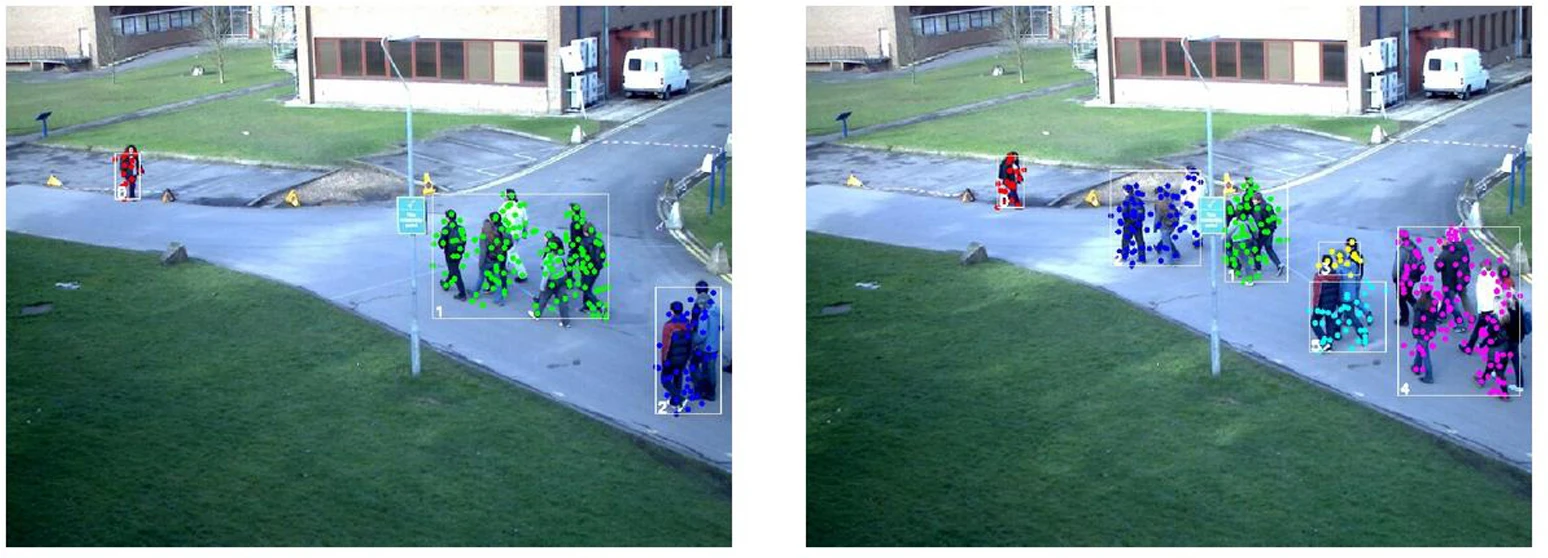
\includegraphics[width=0.8\textwidth]{Figures/history/PETS_CLUSTERS.png}
	\caption{Shlukování SURF bodů v \cite{crowd_on_pets}}
	\label{fig:PETS}
\end{figure}


S narůstající popularitou neuronových sítí v oblasti strojového vidění přirozeně narůstá i množství estimátorů počítajících objekty v obraze, které jsou na neuronových sítích založeny.
Například autoři článku \cite{YOLO_counting} pro tento účel upravili detekční síť YOLO.
Jejich úpravy této sítě spočívaly hlavně v rozdělení obrazu do více buněk a ve větším počtu bounding boxů počítaných pro každou buňku v obraze. Výslednou síť natrénovali tak, ať je citlivá na lidi.
Počet lidí v obraze byl stanoven jako počet bounding boxů, které se nacházely v oblasti, kterou v obraze vytyčili.
Autoři totiž systém zamýšleli pro použití na počítání lidí vycházejících z eskalátoru nebo na jiných místech, kde si mohli být jisti, že lidé budou procházet úzkým prostorem, který bude blízko kamery snímající scénu, takže jednotliví lidé budou v obraze v okamžiku započítání celkem dobře separováni a budou zabírat velké procento scény.
U scén, kde toto není možné by ale nejspíš tento přístup narážel na stejné problémy, jako jiné přímé metody.

Řada nejmodernějších řešení se proto přiklání k nepřímému přístupu počítání objektů v obraze, a to tak, že ze vstupního snímku je vytvořena hustotní mapa, která popisuje odhadovanou hustotu davu v obraze, a výsledný počet lidí v obraze je stanoven na základě této hustotní mapy.
Jednoduchý příklad, jak takovou hustotní mapu vytvořit je uveden v \cite{DeepCorn, Boominathan}.
V trénovacím datasetu jsou označeny místa, kde se nachází jednotlivé hlavy lidí v obrázku obsažených.
Pro každý takový bod je do hustotní mapy vložena Gaussova křivka tak, že \(\mu\) je rovno pozici bodu a obsah pod touto křivkou je roven jedné.
V ideálním případě by byla hodnota \(\sigma\) pro každý bod odvozena od velikosti patřičné hlavy.
Dostupné datasety ale tuto informaci velmi často nemají a pro každou hlavu je známa pouze její pozice. Parametr \(\sigma\) je z toho důvodu často konstantní napříč celou hustotní mapou.
Hodnota každého bodu hustotní mapy je následně získána jako suma všech gaussiánů v daném bodě.
Pokud tuto hustotní mapu zintegrujeme určitým integrálem, tak výsledná hodnota bude rovna počtu lidí, respektive hlav, v daném obraze.
Cílem CNN je tedy naučit se co nejlépe replikovat takto vytvořené hustotní mapy pouze na základě neanotovaných vstupních obrazů.

Mezi takovéto sítě se řadí například M-SFANet \cite{MSFANet_for_crowd_counting}.
Obraz je dán na vstup sítě VGG-16bn \cite{VGG}, která slouží k získání příznaků.
Následně je síť rozdělena na dvě části.
Výstup z desáté vrstvy VGG je dán na vstup modulu CAN (Context-aware module) \cite{CAN_1, CAN_2}, který slouží z získání "scale-aware" příznaků a učí se jejich význam na základě jeho polohy v obraze, což pomáhá, je-li velikost lidí ve vstupním obraze výrazně ovlivněna perspektivou.
Výstup z třinácté vrstvy je vložen na vstup ASPP \cite{ASPP} (Atrous spatial pyramid pooling) modulu, který podobně jako CAN slouží k extrakci "multi scale" příznaků, avšak narozdíl od CAN je důležitost jednotlivých napříč celým obrazem stejná.
Výstupy z těchto modulů jsou vloženy do dvou dekodérů, které slouží vytvoření hustotní a pozornostní mapy (attention map).
Hustotní mapa je vytvořena stejně, jako již výše popsaná, a pozornostní mapa je vytvořena tak, že je-li hodnota v hustotní mapě hodnota větší, než práh, který je stanovený na hodnotu 0,001, tak je hodnota v pozornostní mapě rovna 1, jinak je hodnota rovna 0.
Hadamardův součin těchto map je následně použit jako ground truth pro trénování této sítě.

\begin{figure}[h!]
	\centering
	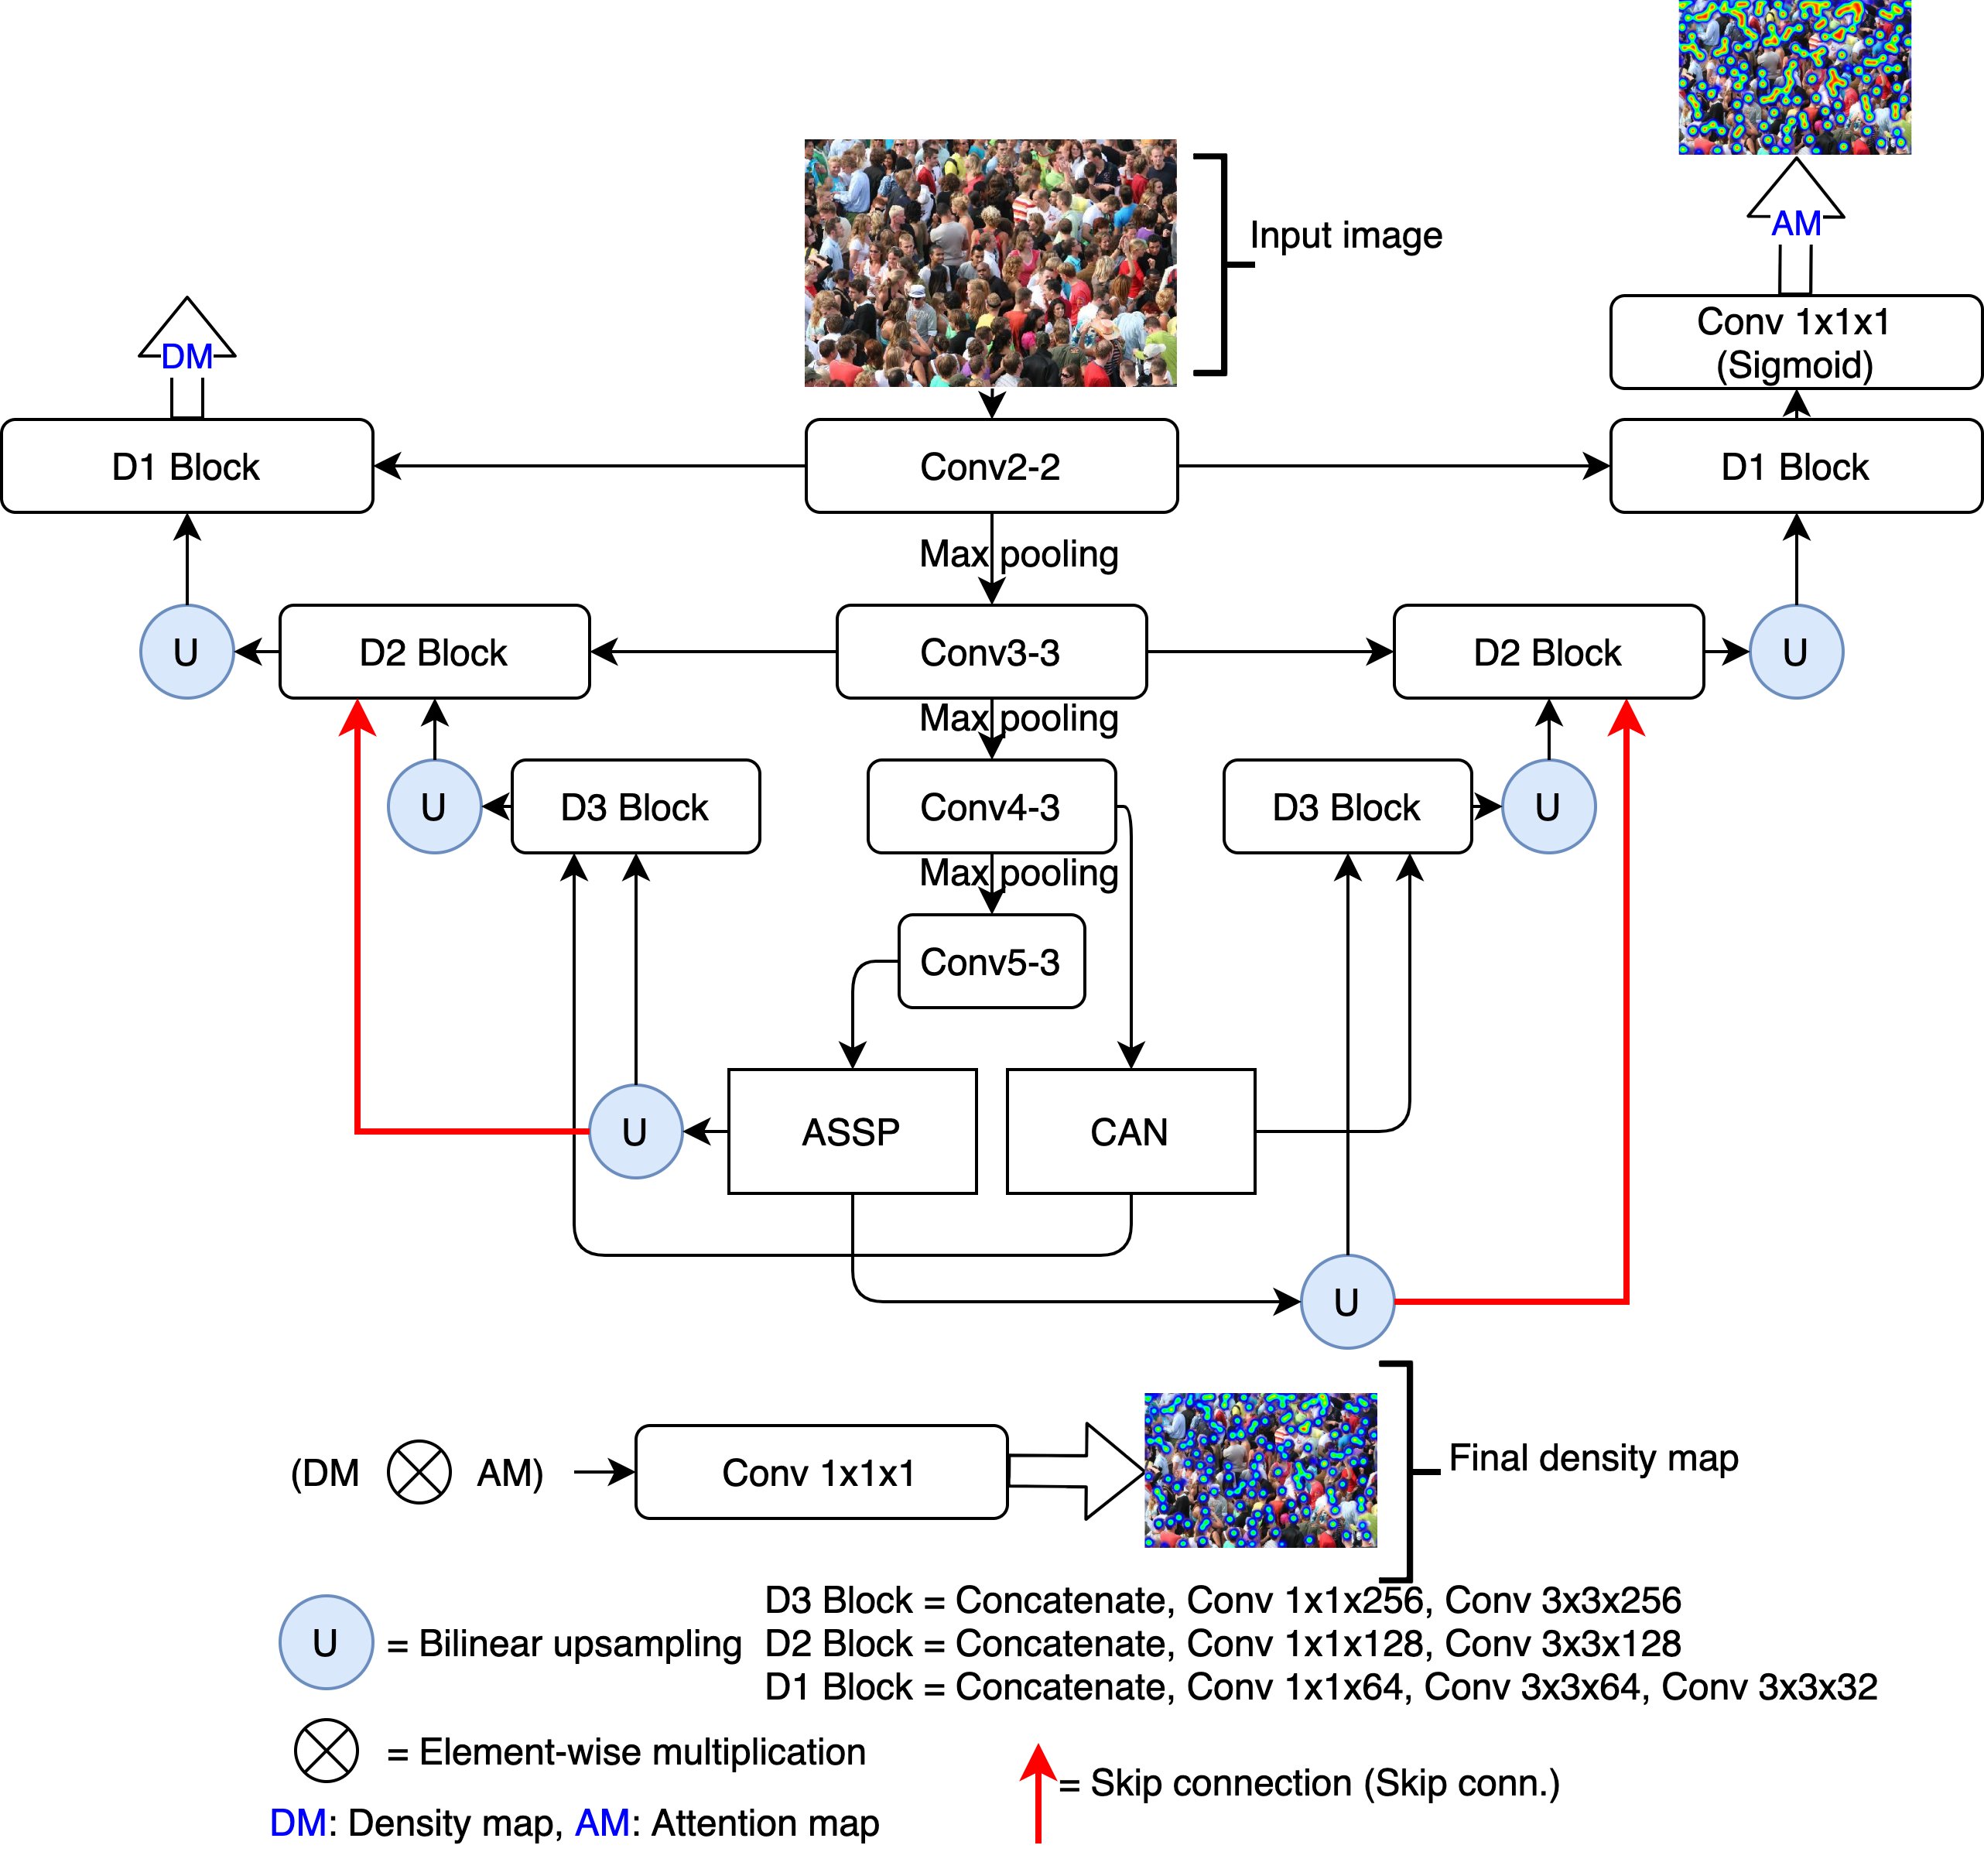
\includegraphics[width=0.6\textwidth]{Figures/history/MSFANet.png}
	\caption{Struktura sítě M-SFANet \cite{MSFANet_for_crowd_counting}}
	\label{fig:M-SFANet}
\end{figure}











\endinput